\section{NetRender}\label{netrender}\index{NetRender}

NetRender is a tool that allows you to render the same image or animation on
multiple computers simultaneously. If you have multiple computers connected to
an Ethernet network, you can greatly increase overall computing power.

One of the computers (server) manages the process of rendering. It sends a
requests to the connected computers (clients) and collects the results of
rendering. Other computers (clients) render different portions of the image and
send it to the server. There can be only one server (master) but clients
(slaves) can be any number. The more clients, the faster the rendering will be.

The Server is also the computer which renders the combined image .

The total number of CPUs (cores) used is the sum of server's CPUs cores + all
client's CPUs cores.

\subsection{Starting NetRender}\label{starting-netrender}

\subsubsection{Server configuration}\label{server-configuration}

On the computer which will be used as the Server, Mode is set to \emph{Server.}

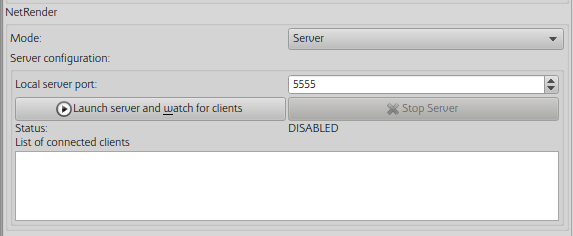
\includegraphics[width=0.7\linewidth]{img/manual/media/netrender_server.png}

\emph{Local server port} should be set to one which is not used by other
applications, and is passed through routers (if any are used) and firewall. The
default is 5555.

If settings are correct, press \emph{Launch server and watch for clients} button
to connect server to existing clients.

At this point, the server is ready to work

Alternative way to launch the server is to use command line. Example:

\begin{verbatim} 
$ mandelbulber2 --server --port 5555 pathToFileToRender.fract
\end{verbatim}

\subsubsection{Configuring the clients}\label{configuring-the-clients}

On the computers which will be used as Clents, \emph{Mode} is set to
\emph{Client}

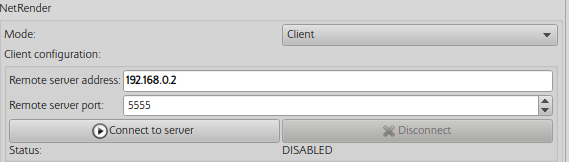
\includegraphics[width=0.7\linewidth]{img/manual/media/netrender_client.png}

The remote server address must be set to the same as the Server computer which
is running Mandelbulber in Server mode. The address can be given as an IP
address or a computer name.

The remote server port number must be exactly the same as the setting on the
Server.

Press \emph{Connect to server} button to connect to the server

Once the connection is established correctly, the client application should show
the status \emph{READY}

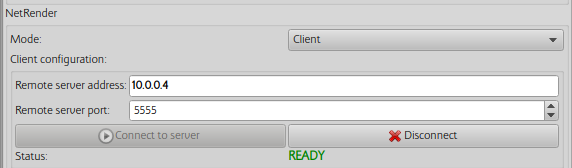
\includegraphics[width=0.7\linewidth]{img/manual/media/netrender_client_connected.png}

Alternative way to establish NetRender client is to use command line:

\begin{verbatim} 
$ mandelbulber2 --nogui --host 10.0.0.4 --port 5555
\end{verbatim}

when connection is successfully established the program should return following
message:

\begin{verbatim} 
NetRender - Client Setup, link to server: 10.0.0.4, port: 5555
NetRender - version matches (2090), connection established 
\end{verbatim}

On the Server computer, in the table "List of connected clients" should be shown
the name and address of the connected clients and the number of available
processors (cores).

i.e ``magda'' computer has 4 cores and is \emph{READY}.

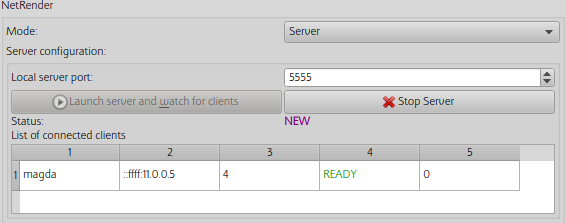
\includegraphics[width=0.7\linewidth]{img/manual/media/netrender_server_connected.png}

\subsubsection{Rendering}\label{rendering}

Only the Server can initiate rendering on the computers connected using
NetRender. When the \emph{RENDER} button is pressed on the server, all the
connected computers commence rendering.

In the table \emph{List of connected clients} in the column \emph{Done lines} will be
shown the number of lines the image rendered by each of the computers.

when rendering is finished, the Server computer, will display the complete
image. On the Client computers, only that portion of the image which was
rendered by that client will be displayed.
